\documentclass[12pt]{article}

\usepackage{fullpage}
\usepackage{graphicx, rotating, booktabs} 
\usepackage{times} 
\usepackage{natbib} 
\usepackage{indentfirst} 
\usepackage{setspace}
\usepackage{grffile} 
\usepackage{hyperref}
\usepackage{adjustbox}
\setcitestyle{aysep{}}


\singlespace
\title{
\textbf{Testing the Public Goods Theory of Alliances}
	}
\author{Joshua Alley\footnote{Graduate Student,
Department of Political Science, Texas A\&M University.}}
\date{{\normalsize \today}}

\bibliographystyle{apsr}

\begin{document}

\maketitle 

\doublespace



%----------------------------------
\section{Introduction}



\citet{OlsonZeckhauser1966} argue that international alliances are subject to a collective action problem. 
Smaller alliance participants ``free ride'' on the contributions of larger members. 
As of November 2018, Olson and Zeckhauser's article has been cited 1670 times.
Furthermore, they argue that collective action dynamics in alliances apply to other international organizations. 
Given its salience and potential implications, this public goods theory of alliances merits careful empirical scrutiny. 


But even after 52 years, we have limited evidence for or against free-riding in alliances. 
Most models are unidentified, and the overwhelming majority of tests focus on NATO. 
The standard test regresses military spending as a share of national income on national income. 
This approach places GDP on both sides of the regression, so the models are unidentified. 


\citet{PluemperNeumayer2015} address the identification problem by examining changes in spending among NATO members. 
In their framework, a lack of responsiveness to US and Soviet military spending is evidence of free riding among NATO members.
They find no correlation between the size of a NATO member and free-riding, which they argue contradicts Olson and Zeckhauser. 
However, they do not include the United States in their sample, which omits a crucial data point for testing the size argument.\footnote{Given the focus on responses to US spending, this decision is understandable.}


% So what is the problem here? 
Despite the canonical status of \citet{OlsonZeckhauser1966}, their predictions have not been subjected to a general, well-identified test. 
Most evidence suggests NATO members spend less on the military thanks to allied capability \citep{PluemperNeumayer2015, GeorgeSandler2017}.
Although NATO is salient, it is the only case with a decent test of free-riding. 


% by the way, it's mostly NATO
We do not know whether the public goods theory of alliances extends beyond NATO. 
My survey of the literature on alliance participation and military spending found six tests of the public goods theory of alliances outside of NATO. 
All six of those studies include GDP in the independent and dependent variable, creating an identification problem. 


% So it total, there's a lot we don't know
Due to identification problems and emphasis on NATO, we have no evidence for the generalizability of the public goods theory of alliances. 
Understanding NATO is worthwhile. 
But it is insufficient to assess the overall explanatory power of the public goods theory of alliances. 


% I'm not the first one to address this theory: first comprehensive empirical evidence
Other scholars have questioned the public goods theory of alliances on theoretical grounds.  
\citet{SandlerHartley2001} summarize several extensions of the argument.  
But such theoretical revisions are premature without knowledge that the more parsimonious public goods model is inappropriate. 
This paper provides the first comprehensive test of the public goods theory of alliances- incorporating multiple alliances over a long time frame. 


% Why we should care
Failures in testing the public goods theory of alliances have two important consequences. 
First, it hinders the accumulation of knowledge. 
Without a valid and comprehensive test, the validity of the public goods theory will remain unclear. 


% Why we should care: policy and free riding
If the public goods theory of alliances was only an academic matter, the lack of solid empirical evidence would be benign. 
But the idea of free-riding is ubiquitous in popular and policy debates. 
Charges of free-riding by NATO members are used to question the value of the treaty itself. 
If the public goods theory of alliances has limited explanatory power, charges of free-riding are on shaky ground. 


Establishing the empirical validity of the public goods theory of alliances is necessary for theoretical progress and policy debates. 
Below, I outline two possible solutions to this challenge. 
Both examine the role of alliance participant size in multiple alliances from 1816 to 2007. 


The first approach uses a standard panel data research design, with an aggregate measure of alliance participation. 
The second design employs a Bayesian model to generate separate estimates for every alliance. 
In the multilevel model, I test Olson and Zeckhauser's prediction that states which contribute more to an alliance should spend more by estimating the impact of increasing alliance contribution on military spending. 
Neither design finds strong evidence for Olson and Zeckhauser's predictions. 


The paper proceeds as follows.
First, I summarize the public goods theory of alliances and translate its predictions into both research designs.
Then, I describe and summarize the results of a panel-data test of the public goods logic.
The third section describes the multilevel model and associated results. 
The final section assesses aggregate support for the public goods logic, as well as implications for scholars and policymakers. 


\section{The Public Goods Theory of Alliances}

% this needs to be succint- aim for 500 words. 

% summarize argument
Why are alliances subject to a public goods problem? 
The aggregate capability of an alliance provides security for members. 
But because a treaty cannot exclude members without undermining its purpose, security is a public good. 


Individual members gain security from treaty participation, regardless of their individual contribution. 
Olson and Zeckhauser expect that larger members of the alliance with bear a higher defense burden, because these states value defense from the alliance more. 
Therefore, smaller alliance members free-ride on the contributions of larger partners. 


% Develop implications for test: one for each section. 
There are two implications of this argument. 
First, we can consider aggregate responses to changes in allied spending by large and small states. 
If Olson and Zeckhauser's argument is correct, smaller states should decrease military spending in response to greater allied military spending. 
Larger states will not respond to increased allied spending. 
This implies a conditional relationship between allied spending, state size, and state military spending. 


\begin{quote}
\textsc{Hypothesis 1}: The marginal effect of allied spending on state military spending will be negative for small states, and decreasing in state size. 
\end{quote}


The other implication deals with differences within individual alliances. 
If larger states bear a disproportionate share of the alliance burden, then within each alliance, increasing contribution should be positively associated with military spending. 
States that contribute more to the alliance will increase military expenditures to maintain the output from the treaty. 


\begin{quote}
\textsc{Hypothesis 2}: Within an alliance, increasing treaty contribution will be positively associated with military spending. 
\end{quote}


Alliances where we observe a positive correlation between treaty contribution and military spending conform to Olson and Zeckhauser's expectations. 
No correlation implies larger members are not increasing military spending.
A negative correlation between treaty contribution and military spending implies larger members are able to decrease spending, which Olson and Zeckhauser's argument cannot explain. 


I now test these two predictions from the public goods theory of alliances in a sample of all states from 1816 to 2007. 
The next section examines Hypothesis 1 by interacting changes in total allied spending and GDP.
This approach aggregates multiple treaties into a single measure of participation. 


\section{Panel Data Regression}

This test of Hypothesis 1 relies on standard measures of state size and alliance participation from prior studies. 
GDP is Olson and Zeckhauser's proxy for state size. 
Total allied capability is a common measure of alliance participation \citep{Sorokin1994, MorganPalmer2003}. 
In this case, I measure total allied capability as the military spending of states with a defensive or offensive treaty with a state. 
The dependent variable is the natural log of military spending \citep{SingerCINC1988}. 


Because the public goods theory of alliances implies a conditional relationship, I specify the following regression model:

\begin{equation} 
y = \beta_1 + \beta_2 \mbox{GDP} + \beta_3 \mbox{Ally Spend} + \beta_4 \mbox{GDP} \times \mbox{Ally Spend} + \beta X 
\end{equation}


$\beta_2$ and $\beta_3$ are the constituent terms and $X$ is a matrix of control variables with coefficient vector $\beta$.
Hypothesis 1 implies $\beta_2$ should be positive, and $\beta$ three should be negative. 
The interaction term $\beta_4$ should be positive. 


I estimate this model using robust regression estimator. 
Even after the log transformation, military spending produces heavy-tailed residuals, so OLS is inefficient \citep{RaineyBaissa2018}. 
Robust regression re-weights observations according to the size of the residual, making it less sensitive to large deviations than OLS. 


In the robust regression, I control for several correlates of alliance participation and military spending. 
First, I include a lagged dependent variable to address temporal autocorrelation.\footnote{Therefore, the model functionally estimates changes in spending}.
I control for international war \citep{Reiteretal2016}, civil war participation \citep{SarkeesWayman2010}, and a count of annual MIDs \citep{Gibleretal2016}. 
Other controls address salient alliance characteristics, including average democracy and number of members across a state's alliance treaties.   
Last, I control for regime type, external threat \cite{LeedsSavun2007}, and Cold War years. 


\subsection{Results}


Estimates from this model do not match Hypothesis 1. 
\autoref{tab:rreg-res} summarizes results from the robust regression estimator. 
As expected, GDP is positively correlated with military spending. 
Changes in allied spending have no effect on military spending, however. 
The interaction term of changes in allied spending and GDP is also statistically insignificant. 

\begin{table}[ht]
\centering
\begin{tabular}{lrrr}
  \hline
 & Value & Std. Error & t value \\ 
  \hline
	Change Allied Spending & -0.020 & 0.044 & -0.453 \\ 
	ln(GDP) & 0.012 & 0.002 & 6.161 \\ 
	Change Allied Spending $\times$ ln(GDP) & 0.001 & 0.002 & 0.805 \\ 
  Lag ln(Military Spend.) & 0.992 & 0.001 & 805.703 \\ 
  Avg Alliance Size & 0.001 & 0.000 & 4.370 \\ 
  Avg Alliance Democracy & -0.001 & 0.001 & -1.547 \\ 
  International War & 0.090 & 0.010 & 9.396 \\ 
  Civil War Participation & 0.005 & 0.007 & 0.717 \\ 
  Polity & -0.000 & 0.000 & -0.777 \\ 
  International Threat & 0.026 & 0.011 & 2.437 \\ 
  Cold War & 0.046 & 0.004 & 11.472 \\
	Constant & -0.180 & 0.038 & -4.690 \\ 
   \hline
\end{tabular}
\caption{Robust Regression Estimates: Allied Spending, GDP, and military spending 1816-2007.}
\label{tab:rreg-res}
\end{table}


Interactions cannot be interpreted using the coefficients alone \citep{BramborClarkGolder2006}. 
\autoref{fig:abs-margins-plot} plots the marginal effect of allied military spending across the distribution of GDP. 
The marginal effect of allied military spending is never negative. 
There is no discernible interaction between state size and changes in allied spending. 

\begin{figure}
	\centering
		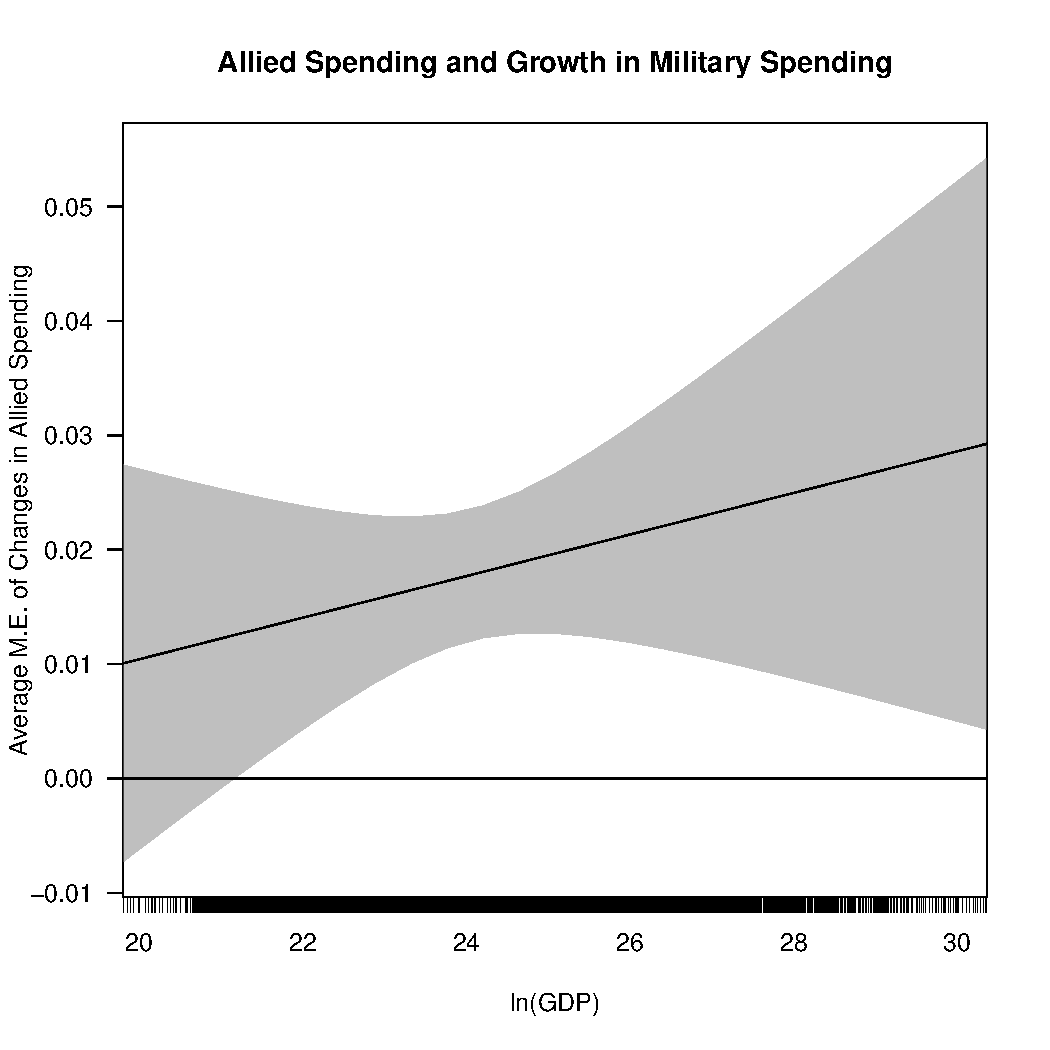
\includegraphics[width=0.95\textwidth]{abs-margins-plot.pdf}
	\label{fig:abs-margins-plot}
	\caption{Average Marginal Effect of increasing allied military spending on a state's military spending, across the range of GDP.}
\end{figure}


These results are robust to an OLS estimator, and kernel estimation of the interactive relationship \citep{Hainmuelleretal2017}. 
I also estimated a model that treats states with an alliance as the estimation sample, and used the Heckman two-stage estimator to address potential non-random selection into alliances. 
None of these estimates match the expectations of Hypothesis 1. 


Of course, it is possible that by aggregating multiple alliance treaties into a single measure, this regression does not capture heterogeneous effects of individual treaties.
Small states could make a large contribution to an alliance if their partner is even smaller. 
So the next section examines how many alliances match the expectations of the public goods theory. 


\section{Multilevel Model}


Testing Hypothesis 2 requires estimating a unique parameter for each alliance.
For each of the 285 alliances that promise military support, I estimate the association between increasing treaty contribution and military spending. 
Bayesian estimation is well-suited to this kind of estimation problem, so I fit the following model using STAN \citep{Carpenteretal2016}.

The full model is starts with state-year changes in the natural log of military spending $y_{it}$.
I model the DV with a t-distribution to account for heavy tails.
$\nu$ is the degrees of freedom parameter- as $\nu$ increases, the t distribution becomes more like a normal distribution. 


\begin{equation}
y_{it} \sim student_t(\nu, \mu, \sigma) 
\end{equation}


Otherwise, the model is a fairly typical regression model.
The expected value of the outcome $\mu_{it}$ depends on a constant $\alpha$, state and year varying intercepts $\alpha^{st}$ and $\alpha^{yr}$, a lagged DV $y_{t-1}$, and control variables $X_{it} \beta$. 
In this specification, I include all the non-alliance controls from the first robust regression in $X$.


\begin{equation}
\mu_{it} = \alpha + \alpha^{st} + \alpha^{yr} + \eta y_{t-1} + X_{it} \beta + Z_{it} \lambda 
\end{equation}


The $Z_{it} \lambda$ term captures the potential impact of multiple alliances. 
$Z$ is a matrix of state participation in alliances--- columns are alliances, rows are state-year observations. 
If a state is not in an alliance, the corresponding element of the matrix is equal to zero. 
If a state is part of an alliance, the corresponding element of the matrix is equal to a state's military spending as a share of allied spending. 
The alliance contribution elements of the matrix range from 0 to 1, because some states have no military spending.\footnote{Costa Rica is the best-known example of this.} 


$\lambda$ is a vector of alliance-specific parameters.  
There are 285 alliances, each with a unique posterior of $\lambda$. 
These parameters capture the association between treaty contribution and military spending. 
A positive $\lambda$ implies that as contribution to the alliance increases, members spend more. 


When a state is not in an alliance, the corresponding $\lambda$ is multiplied by zero, and has no impact. 
So only alliances a state contributes to affect military expenditures. 
Each alliance a state is a member of has a separate impact on military spending.
Thus, all alliance estimates hold the impact of other treaties constant.     


\subsection{Results} 


If the public goods theory of alliances is correct, we should observe many positive $\lambda$ parameters. 
Because I estimated this model in the Bayesian framework, each $\lambda$ has a posterior distribution.\footnote{See the appendix for a full summary of priors, convergence and model fit.} 
Interpretation focuses on the posterior mean and 90\% credible intervals.\footnote{I use the 90\% credible intervals because inferences around the 95\% intervals can be less stable.}
The posterior mean is the expected value of $\lambda$, while the credible intervals capture uncertainty around that estimate.  


\begin{figure}[htbp]
	\centering
		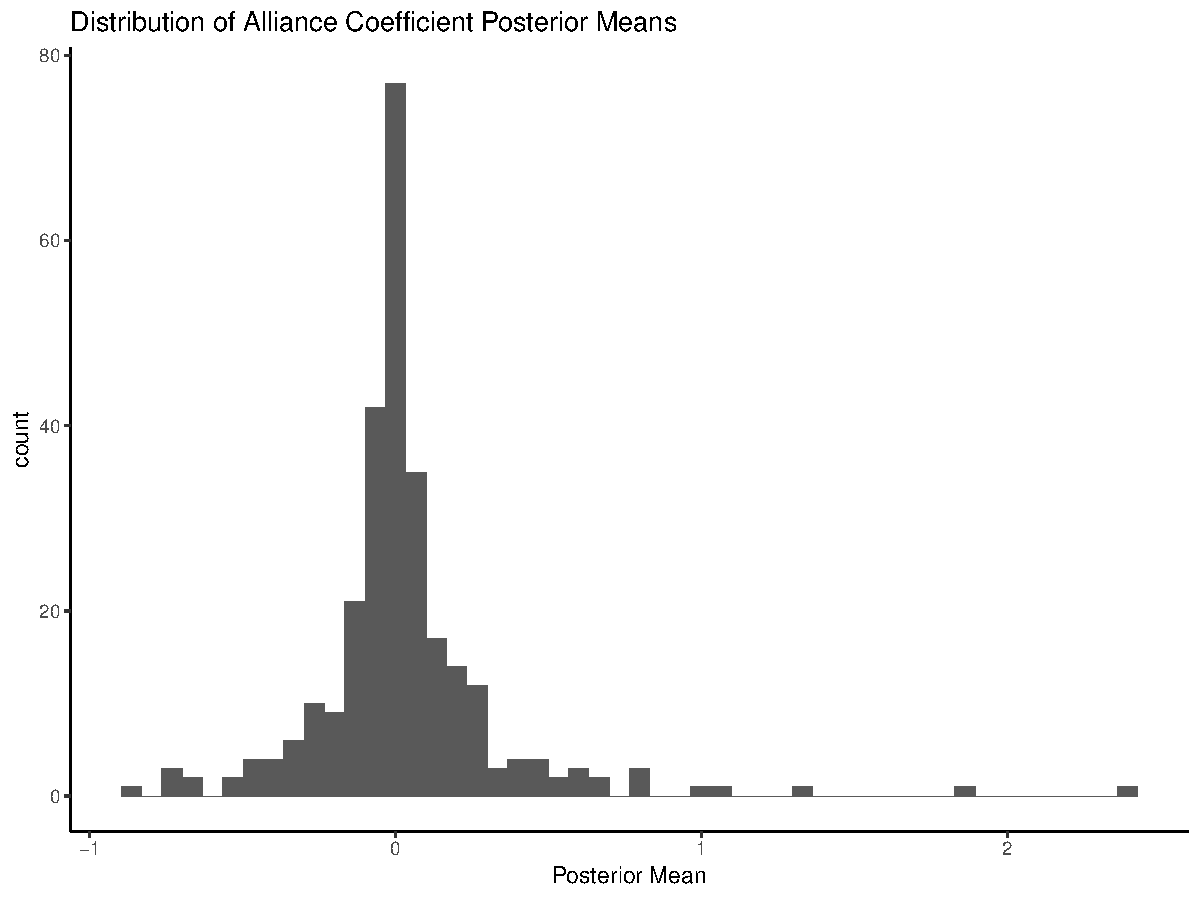
\includegraphics[width=0.95\textwidth]{alliance-coefs-hist.pdf}
	\caption{Posterior mean of association between alliance contribution and military spending in 285 defensive and offensive alliances from 1816 to 2007.}
	\label{fig:alliance-coefs-hist}
\end{figure}


\autoref{fig:alliance-coefs-hist} summarizes the posterior mean of the 285 alliance coefficients. 
The distribution is strongly concentrated around zero. 
There are large positive values, but also a good number of large negative values.


In total, 141 of 285 alliances have a positive posterior mean. 
144 of 285 alliances have a negative posterior mean. 
The large number of negative values is some evidence against the prediction of Hypothesis 2. 
However, the posterior means do not convey whether the impact of increasing alliance contribution can be distinguished from zero. 
Plotting the posterior mean and credible intervals provides a succint summary. 


\autoref{fig:alliance-coefs-year} plots the $\lambda$ parameter for each alliance against the start year of the treaty.
Each point is the posterior mean. 
The error bars summarize the 90\% credible interval.\footnote{The credible intervals summarize the 5\% and 95\% quantiles of the posterior.}  


\begin{figure}[htbp]
	\centering
		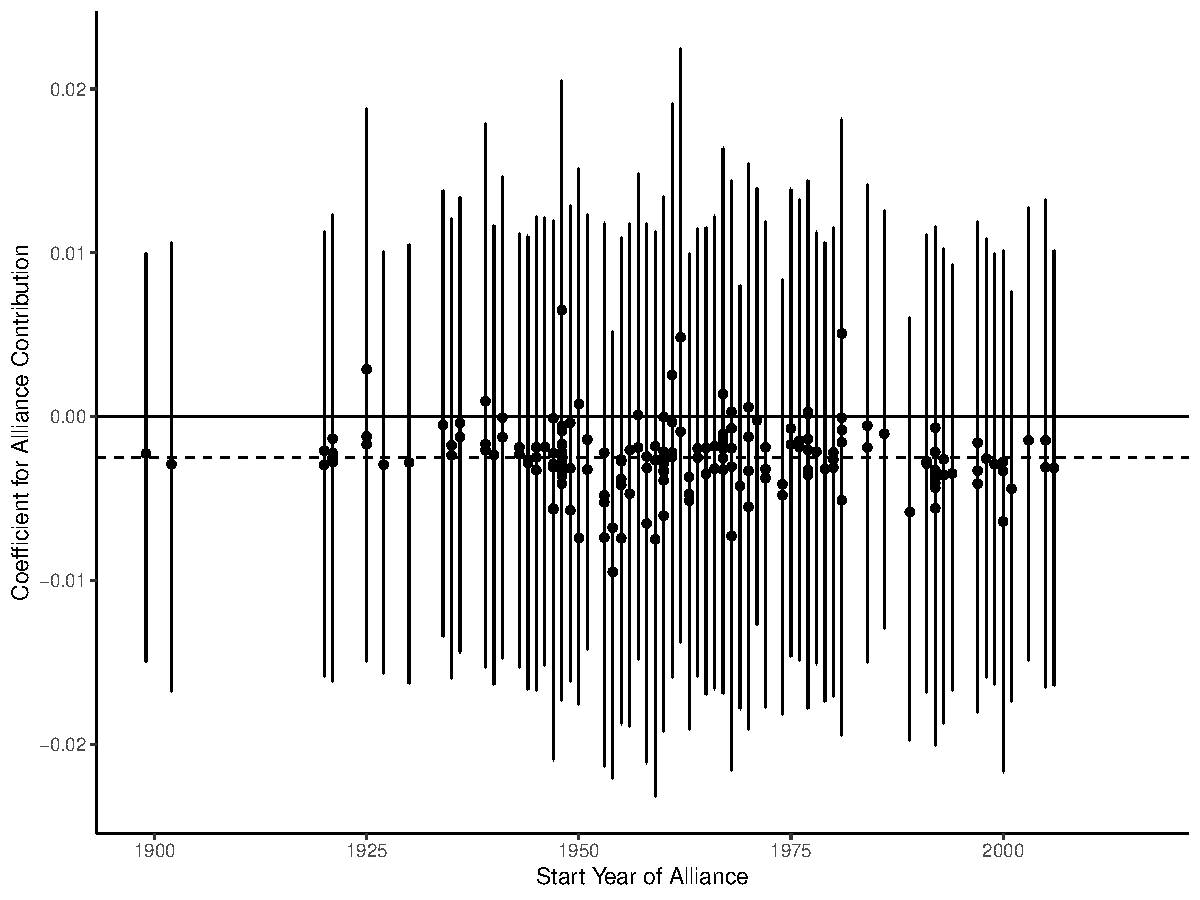
\includegraphics[width=0.95\textwidth]{alliance-coefs-year.pdf}
	\caption{Estimated association between alliance contribution and defense spending in 285 defensive and offensive alliances from 1816 to 2007. Points represent the posterior mean and the error bars cover the 90\% credible interval.}
	\label{fig:alliance-coefs-year}
\end{figure}


Because many of the posterior means are close to zero, 251 credible intervals include zero. 
There are 20 alliances where the credible interval includes only positive values. 
That leaves 14 treaties where the credible interval covers only negative values. 


20 of 285, or 7\%, is a dismal prediction success rate for Hypothesis 2. 
There is no association between treaty contribution and military spending in most alliances.
The 14 negative $\lambda$ parameters imply larger members of those alliances \emph{spend less} on the military, which the public goods theory cannot explain. 


NATO, the best-studied case for the public goods, offers no support for the public goods theory of alliances. 
The posterior mean is $-0.004$, and the credible interval ranges from -.26 to .26.  
Greater contribution to NATO is not associated with increased military spending. 
This finding corroborates the results of \citet{PluemperNeumayer2015}. 
This may reflect how this model controls for membership in other alliances, which prior studies were unable to. 


% Maybe add the figure with non-zero alliances?: check space.  


This second set of estimates provides little support for predictions from the public goods theory of alliances. 
In 88\% of alliances, there is no association between treaty contribution and military spending. 
Taken in conjunction with the single-level results, there is little empirical support for the public goods theory of alliances.


\section{Conclusion}


These findings imply that we should treat the public goods model of alliances with caution. 
Olson and Zeckhauser's model is simple and intuitive, but it lacks explanatory power. 
Better identified empirical models and examination of multiple treaties shows little evidence small states leave larger counterparts to bear a higher burden. 


My results reinforce extant theoretical skepticism about the public goods model. 
\citet{Palmer1990} and \citet{SandlerHartley2001} provide two theoretical critiques that may merit further scrutiny. 
Constructing parsimonious models of alliances and defense effort is the next challenge. 
Components of the public goods model and these alternatives may provide a useful starting point. 


Some of the results raise additional questions for theoretical work. 
Why do we observe 14 alliances where increasing alliance contributions are associated with reduced spending?
Why is the effect of greater allied spending mostly positive? 


Furthermore, scholars should reassess the concept of ``free-riding'' in alliance politics. 
Free-riding is closely tied to public goods, so limited validity for a public goods approach may limit the validity of free-riding. 
Charges of free-riding are normatively loaded and may mask significant exchanges between alliance members \citep{Lanoszka2015}. 


This is not a call to abandon the public goods model in international politics more generally. 
The public goods model may still apply to other international organizations. 
It has limited explanatory power across alliances, however. 


Despite concerns about its explanatory power, the public goods model of alliances has a salient role in discussions of alliance participation and defense effort. 
I find little evidence that reduced military spending by alliance members is the result of a collective action problem. 
Public goods models are useful in many contexts, but they have little explanatory power in alliance politics. 


\singlespace


%\bibliography{C:/Users/jkalley14/Dropbox/Research/MasterBibliography}  
\bibliography{C:/Users/Josh/Dropbox/Research/MasterBibliography} 





\end{document}


